% Figure: Citation Distribution across the Sutra Corpus
% Data source: Sutra Pipeline database, 17,956 high-relevance papers
% Usage: % Figure: Citation Distribution across the Sutra Corpus
% Data source: Sutra Pipeline database, 17,956 high-relevance papers
% Usage: % Figure: Citation Distribution across the Sutra Corpus
% Data source: Sutra Pipeline database, 17,956 high-relevance papers
% Usage: % Figure: Citation Distribution across the Sutra Corpus
% Data source: Sutra Pipeline database, 17,956 high-relevance papers
% Usage: \input{figures/citation-distribution.tex}

\begin{figure}[t]
\centering
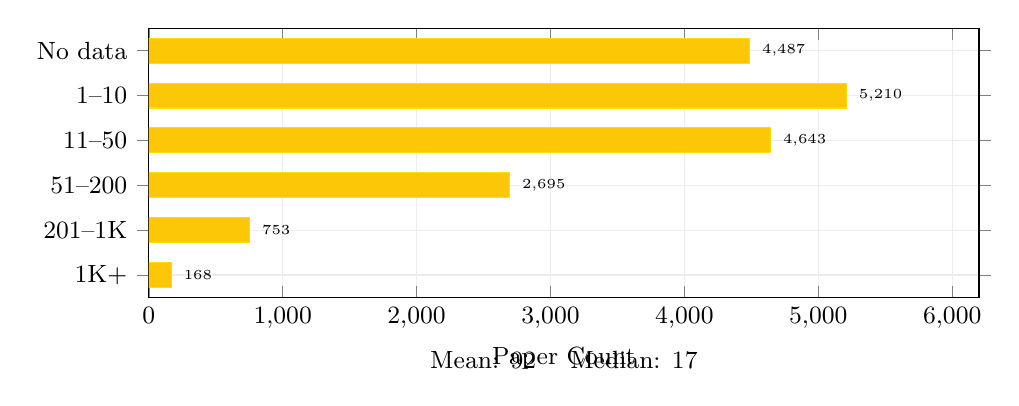
\begin{tikzpicture}
\begin{axis}[
    xbar,
    width=\columnwidth,
    height=5cm,
    xlabel={Paper Count},
    xlabel style={font=\small},
    xmin=0, xmax=6200,
    ytick=data,
    yticklabels={
        {No data},
        {1--10},
        {11--50},
        {51--200},
        {201--1K},
        {1K+}
    },
    yticklabel style={font=\small},
    y dir=reverse,
    bar width=9pt,
    nodes near coords,
    nodes near coords style={font=\tiny, anchor=west},
    every node near coord/.append style={xshift=1pt},
    enlarge y limits={abs=0.5},
    grid=major,
    grid style={gray!15},
    xticklabel style={font=\small},
    point meta=explicit symbolic,
    title={\small Mean: 92 \quad Median: 17},
    title style={at={(0.5,0)}, anchor=north, yshift=-22pt},
]
\addplot[fill=yellow!60!orange, draw=yellow!80!orange] coordinates {
    (4487,0) [4{,}487]
    (5210,1) [5{,}210]
    (4643,2) [4{,}643]
    (2695,3) [2{,}695]
    (753,4)  [753]
    (168,5)  [168]
};
\end{axis}
\end{tikzpicture}
\caption{\textbf{Citation distribution} across the Sutra Corpus.
The power-law shape (mean 92, median 17) reflects a small number of
foundational papers accumulating thousands of citations while most
have modest impact.}
\label{fig:cite-distribution}
\end{figure}


\begin{figure}[t]
\centering
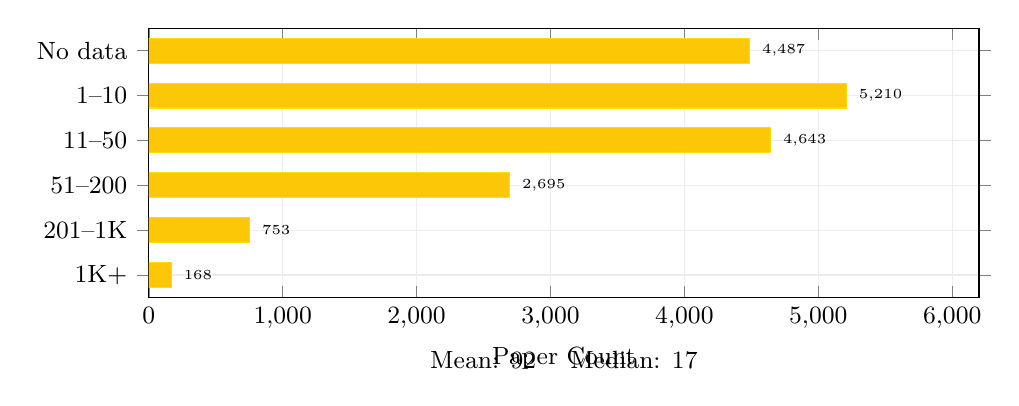
\begin{tikzpicture}
\begin{axis}[
    xbar,
    width=\columnwidth,
    height=5cm,
    xlabel={Paper Count},
    xlabel style={font=\small},
    xmin=0, xmax=6200,
    ytick=data,
    yticklabels={
        {No data},
        {1--10},
        {11--50},
        {51--200},
        {201--1K},
        {1K+}
    },
    yticklabel style={font=\small},
    y dir=reverse,
    bar width=9pt,
    nodes near coords,
    nodes near coords style={font=\tiny, anchor=west},
    every node near coord/.append style={xshift=1pt},
    enlarge y limits={abs=0.5},
    grid=major,
    grid style={gray!15},
    xticklabel style={font=\small},
    point meta=explicit symbolic,
    title={\small Mean: 92 \quad Median: 17},
    title style={at={(0.5,0)}, anchor=north, yshift=-22pt},
]
\addplot[fill=yellow!60!orange, draw=yellow!80!orange] coordinates {
    (4487,0) [4{,}487]
    (5210,1) [5{,}210]
    (4643,2) [4{,}643]
    (2695,3) [2{,}695]
    (753,4)  [753]
    (168,5)  [168]
};
\end{axis}
\end{tikzpicture}
\caption{\textbf{Citation distribution} across the Sutra Corpus.
The power-law shape (mean 92, median 17) reflects a small number of
foundational papers accumulating thousands of citations while most
have modest impact.}
\label{fig:cite-distribution}
\end{figure}


\begin{figure}[t]
\centering
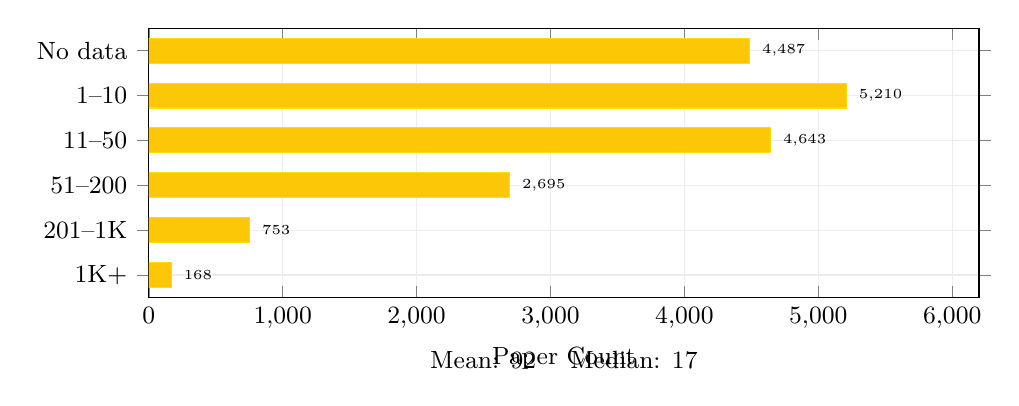
\begin{tikzpicture}
\begin{axis}[
    xbar,
    width=\columnwidth,
    height=5cm,
    xlabel={Paper Count},
    xlabel style={font=\small},
    xmin=0, xmax=6200,
    ytick=data,
    yticklabels={
        {No data},
        {1--10},
        {11--50},
        {51--200},
        {201--1K},
        {1K+}
    },
    yticklabel style={font=\small},
    y dir=reverse,
    bar width=9pt,
    nodes near coords,
    nodes near coords style={font=\tiny, anchor=west},
    every node near coord/.append style={xshift=1pt},
    enlarge y limits={abs=0.5},
    grid=major,
    grid style={gray!15},
    xticklabel style={font=\small},
    point meta=explicit symbolic,
    title={\small Mean: 92 \quad Median: 17},
    title style={at={(0.5,0)}, anchor=north, yshift=-22pt},
]
\addplot[fill=yellow!60!orange, draw=yellow!80!orange] coordinates {
    (4487,0) [4{,}487]
    (5210,1) [5{,}210]
    (4643,2) [4{,}643]
    (2695,3) [2{,}695]
    (753,4)  [753]
    (168,5)  [168]
};
\end{axis}
\end{tikzpicture}
\caption{\textbf{Citation distribution} across the Sutra Corpus.
The power-law shape (mean 92, median 17) reflects a small number of
foundational papers accumulating thousands of citations while most
have modest impact.}
\label{fig:cite-distribution}
\end{figure}


\begin{figure}[t]
\centering
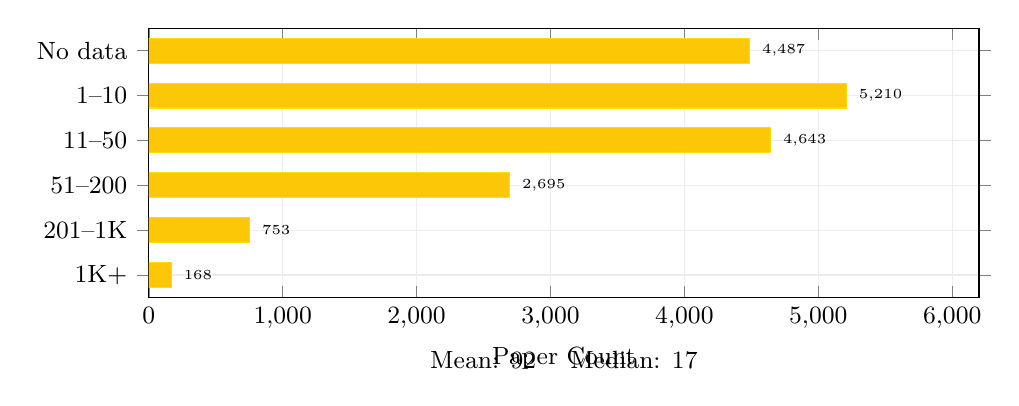
\begin{tikzpicture}
\begin{axis}[
    xbar,
    width=\columnwidth,
    height=5cm,
    xlabel={Paper Count},
    xlabel style={font=\small},
    xmin=0, xmax=6200,
    ytick=data,
    yticklabels={
        {No data},
        {1--10},
        {11--50},
        {51--200},
        {201--1K},
        {1K+}
    },
    yticklabel style={font=\small},
    y dir=reverse,
    bar width=9pt,
    nodes near coords,
    nodes near coords style={font=\tiny, anchor=west},
    every node near coord/.append style={xshift=1pt},
    enlarge y limits={abs=0.5},
    grid=major,
    grid style={gray!15},
    xticklabel style={font=\small},
    point meta=explicit symbolic,
    title={\small Mean: 92 \quad Median: 17},
    title style={at={(0.5,0)}, anchor=north, yshift=-22pt},
]
\addplot[fill=yellow!60!orange, draw=yellow!80!orange] coordinates {
    (4487,0) [4{,}487]
    (5210,1) [5{,}210]
    (4643,2) [4{,}643]
    (2695,3) [2{,}695]
    (753,4)  [753]
    (168,5)  [168]
};
\end{axis}
\end{tikzpicture}
\caption{\textbf{Citation distribution} across the Sutra Corpus.
The power-law shape (mean 92, median 17) reflects a small number of
foundational papers accumulating thousands of citations while most
have modest impact.}
\label{fig:cite-distribution}
\end{figure}
